\subsection{Visão Geral}\label{2-fundamentacao-dbs-visao-geral}

Os sistemas computacionais possuem um papel cada vez mais relevante no suporte às atividades (de negócio) de uma organização. O desenvolvimento de um sistema computacional é uma tarefa não trivial. Além da identificação dos requisitos funcionais de um sistema, cada vez mais as equipes de desenvolvimento se veem confrontadas com a necessidade de suporte a um conjunto cada vez maior de requisitos não funcionais, tais como segurança, escalabilidade, disponibilidade e interoperabilidade. Adicionalmente, as necessidades do acesso ao sistema por usuários geograficamente distribuídos contribuem para aumentar a complexidade destes sistemas.

A arquitetura de um sistema computacional descreve as propriedades fundamentais de um sistema em seu ambiente de execução em termos de seus elementos (componentes), relacionamentos e princípios que norteiam o desenvolvimento e a evolução deste sistema~\cite{IEEE-2011-ARQUITETURA}. A descrição da arquitetura de um sistema é utilizada como base para seu projeto, seu desenvolvimento e sua manutenção.

O Desenvolvimento Baseado em Serviços (DBS), também chamado de Arquitetura Orientada a Serviços (\textit{Service Oriented Architecture} – SOA)~\cite{PAPAZOGLOU-GEORGAKOPOULOS-2003-Service-Oriented-Computing, VALIPOUR-AMIRZAFARI-MALEKI-DANESHPOUR-2009-SOA}, é um paradigma de desenvolvimento de software que facilita o projeto, o desenvolvimento, a manutenção e a evolução de um sistema computacional. De acordo com esse paradigma, serviços representam os elementos fundamentais no desenvolvimento de uma nova aplicação.

%Nos últimos 15 anos, presenciamos o surgimento de um novo paradigma de desenvolvimento de software chamado Desenvolvimento Baseado em Serviços (DBS) ou, alternativamente, Arquitetura Orientada à Serviços (\textit{Service Oriented Architecture} – SOA)~\cite{PAPAZOGLOU-GEORGAKOPOULOS-2003-Service-Oriented-Computing, VALIPOUR-AMIRZAFARI-MALEKI-DANESHPOUR-2009-SOA}. De acordo com esse paradigma, serviços representam os elementos fundamentais no desenvolvimento de uma nova aplicação.

Um serviço consiste em uma entidade de software (componente) aberta, com interface bem definida e cujas funcionalidades podem ser acessadas (remotamente) por entidades clientes. Uma descrição de serviço é utilizada para definir as funcionalidades e o comportamento esperado de um serviço, bem como os detalhes técnicos necessários à localização do serviço e à invocação de suas funcionalidades.

Serviços são oferecidos por provedores de serviços e consumidos por clientes de serviços. Um provedor de serviço consiste em uma organização responsável por manter a infraestrutura técnica necessária à execução do serviço, bem como por disponibilizar a descrição do serviço. Um cliente de serviço representa uma entidade que utiliza as funcionalidades de um serviço para atingir seus objetivos. Clientes podem realizar buscas em repositórios públicos contendo descrições de serviços para identificar serviços de interesse. Um serviço pode ser utilizado de forma isolada ou combinada com outros serviços para o rápido desenvolvimento de uma nova aplicação, criando as chamadas composições de serviço.

A \figurename~\ref{fig:arquitetura-orientada-servicos} ilustra os principais elementos de uma arquitetura orientada a serviços. A seta pontilhada representa a publicação de uma descrição de serviço em um repositório público da web, feita por um provedor de serviços. A seta tracejada representa a descoberta de um serviço web, por a de descrições existentes em um dado repositório. Esta descoberta é realizada por um cliente de serviços. Finalmente, a seta sólida representa uma requisição de um serviço, realizada por um cliente de serviço.

%Um provedor de serviços suporta a execução de um conjunto de serviços. Descrições dos serviços suportadas são publicadas em um repositório, o qual pode ser consultado por diferentes clientes para a descoberta de serviços. Clientes de serviços invocam operações em um ou mais serviços de interesse.

Um dos principais objetivos do DBS é disponibilizar as funcionalidades implementadas por diferentes aplicações na forma de serviços, por meio do encapsulamento, da organização e da orquestração dessas funcionalidades. Neste sentido, as diferentes funcionalidades providas por um sistema (existente) podem ser utilizadas como base para o desenvolvimento de diferentes serviços. Um mesmo serviço também pode ser reutilizado no desenvolvimento de novas aplicações. Adicionalmente, o DBS provê suporte à interoperabilidade, por meio do uso de descrições de serviço padronizadas e independentes de linguagens de programação e do uso de protocolos abertos para permitir a interação entre as entidades clientes e os serviços propriamente ditos.


\begin{figure}[h]
    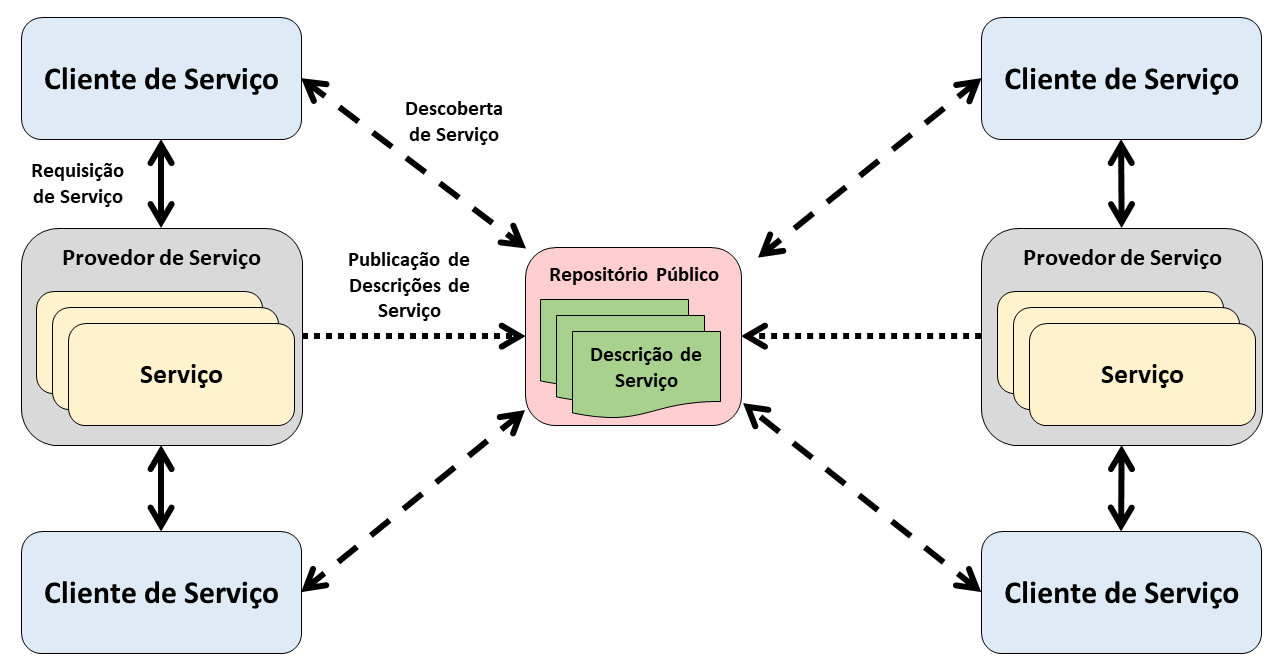
\includegraphics[scale=0.45]{2-fundamentacao-teorica/imagens/arquitetura-orientada-a-servicos(1).png}
    \centering
    \caption[Arquitetura orientada à serviços.]{\textbf{Arquitetura orientada a serviços.}}
    \label{fig:arquitetura-orientada-servicos}
\end{figure}